\documentclass[11pt, twocolumn]{article}
\usepackage[margin=1in]{geometry}
\usepackage[onehalfspacing]{setspace}
\usepackage{lipsum}
\usepackage{flushend}
\usepackage{multicol}
\DeclareUnicodeCharacter{202F}{\,}

\usepackage[
    backend=biber,
    maxnames=20,
    style=nature,
    defernumbers=true
]{biblatex}
\addbibresource{references.bib}

\usepackage{amsmath}
\usepackage{physics}
\usepackage{bm}
\usepackage{graphicx}
\usepackage{hyperref}

\usepackage{titling}
\newcommand \myabstract[2][.8]{%
  \renewcommand\maketitlehookd{%
    \mbox{}\medskip\par
    \centering
    \begin{minipage}{#1\textwidth}
      #2
    \end{minipage}}} 

\begin{document}

\author{Qile Yang}
\title{BIO ENG C142: Final Project Report}
\date{\today}
\myabstract{I introduce a streamlined machine-learning potential that delivers density-functional accuracy for small CHON molecules at force-field speed. Using the ANI Atomic Environment Vector descriptor and TorchANI, I trained element-specific feed-forward networks on a curated GDB subset. An architecture sweep identified a single-hidden-layer model (128 neurons per element; 197K parameters) as the best. With Adam optimisation, the model attains an RMSE of 1.03 kcal on an unseen test set while retaining laptop-scale training (~minutes on an RTX 3050). ReLU activations outperformed CELU variants. Overall, a much more compressed model than the original ANI-1 potential was achieved, with a similar performance on the small organic molecule dataset.}

\maketitle

\section{Introduction}

Understanding and predicting the behavior of molecules and materials at the atomic level is fundamental to advancements across various scientific disciplines, including drug discovery, materials science, and catalysis \cite{wang2018silico, dominy2004native, cicaloni2019applications}. Accurate computational modeling allows researchers to explore chemical space, predict reaction outcomes, and design novel functional materials without the need for costly and time-consuming physical experiments.

At the heart of highly accurate computational methods lies quantum mechanics. Density Functional Theory (DFT) is a prominent approach that offers a favorable balance between accuracy and computational tractability for many systems \cite{engel2011density}. Instead of solving the complex many-body Schrödinger equation directly, DFT cleverly recasts the problem in terms of the electron density, $\rho(\mathbf{r})$. The core idea is that the ground state energy and all other ground state properties are unique functionals of the ground state electron density, $E_0 = E[\rho_0]$. In practice, DFT often relies on solving the Kohn-Sham equations, a set of single-particle equations that yield the electron density of the interacting system.

Despite the successes of DFT, a significant challenge remains in balancing computational accuracy with efficiency. The computational cost of DFT calculations scales cubically, limiting its application to relatively small systems or short simulation timescales \cite{engel2011density, cohen2012challenges}. Conversely, classical force fields, which use simplified, empirically parameterized functions to describe interatomic interactions, offer computational efficiency suitable for large-scale simulations (millions of atoms) and long timescales. However, these force fields often lack the necessary accuracy and transferability, especially for systems involving chemical reactions, complex electronic effects, or environments significantly different from those used in their parameterization \cite{herbers2013grand}.

To address the computational drawbacks, many machine-learning based approaches offer massive speedups. One landmark approach encodes molecules with an Atomic Environment Vector (AEV) representation, developed as part of the ANI framework, specifically the ANI-1 potential described by Smith et al.. \cite{smith2017ani} The ANI-1 potential and its associated AEVs demonstrated the ability to achieve near-DFT accuracy for predicting molecular energies and forces but at a significantly reduced computational expense, comparable to traditional force fields. The AEVs provide a fixed-size, symmetry and permutation-invariant descriptor of an atom's local chemical environment, making them suitable inputs for simpler neural network models by essentially enforcing a hard prior that the local environment contains all relevant energy information. The approach has been shown to be effective and easily extensible for a wide range of molecular systems, including organic molecules and biomolecules, and has been improved for larger systems and applications. \cite{devereux2020extending}

Here, I try to refine the existing ANI-1 potential to improve its performance on a specific class of molecules, namely, small organic molecules. I use the ANI potential as inspiration to adapt different model architectures to a subset of the GDB dataset \cite{ruddigkeit2012enumeration} comprised only of small molecules with the atoms Hydrogens, Oxygens, Carbons, and Nitrogens. The goal is to achieve a more accurate and efficient model for predicting molecular properties, particularly for small organic molecules.

\section{Methods}

I explored several neural network architectures and training strategies to refine the ANI potential for small organic molecules. The primary goal was to enhance the model's ability to predict molecular properties with higher accuracy while maintaining computational efficiency. To achieve this, I experimented with a variety of architectural modifications and training methodologies. All models were trained using the exact same atomic environment vector (AEV) representation implemented with the torchani package. \cite{gao2020torchani} The output of the model was a single scalar value representing the predicted molecular energy.

All architectures were built to be duplicated for use on each atom. The main ones tested included the incorporation of multi-head self-attention layers \cite{vaswani2017attention} before feedforward layers to capture complex and long-range interactions in the atomic environment. Residual connections were also evaluated to facilitate gradient flow and mitigate the vanishing gradient problem, which is particularly important for deeper networks. Various activation functions were also evaluated, including ReLU, GELU \cite{hendrycks2016gaussian}, and CELU, to determine their impact on model performance and convergence speed.

The dataset used for training and evaluation was split into 80\% training, 10\% validation, and 10\% testing to ensure a fair evaluation of the model's performance. To further enhance the robustness of the evaluation process and mitigate overfitting, I employed K-Fold cross-validation with $k=3$. This approach allowed the model to be trained and validated on multiple subsets of the data, providing a more comprehensive assessment of its generalization capabilities.

 The primary evaluation metric for the models was the Mean Absolute Error (MAE) in kcal/mol, which directly reflects the accuracy of the predicted molecular energies. This metric was chosen because it provides an intuitive measure of the average deviation between predicted and true values, making it suitable for assessing the performance of regression models in this domain.

All training was conducted using the Adam optimizer, which is well-suited for handling sparse gradients and adaptive learning rates. Hyperparameters, including batch size, learning rate, number of epochs, and L2 regularization strength, were manually tuned through an iterative process to optimize the model's performance. Early stopping was employed based on the validation loss to prevent overfitting and ensure that the model did not continue training once its performance on unseen data began to degrade.

To accelerate computation and enable the training of more complex models, all computations were conducted on an NVIDIA RTX3050 laptop GPU through a windows subsystem for linux on the x86-64 architecture with 32GB of RAM. This setup provided sufficient computational power to handle the dataset and the computational demands of training neural networks of this. The final model was selected based on the lowest validation MAE observed during training. Once selected, the model was evaluated on the held-out test set to report its performance, ensuring that the reported results reflect its ability to generalize to unseen data. I also investigated the effect of replacing ReLU with a continuous alternative, CELU, to see if the model's performance and convergence speed could be improved.

\section{Results}

The best model architecture was a set of four identical but parameter-wise independent simple Feedforward networks (one for each species) with a single hidden layer of 128 weights that used a ReLU activation function, making up 197636 learnable parameters in total. The hyperparameter combination that used were a batch size of 2048, a learning rate of 0.0001, 100 epochs of training, and 0 regularization.

\begin{figure}[h]
    \centering
    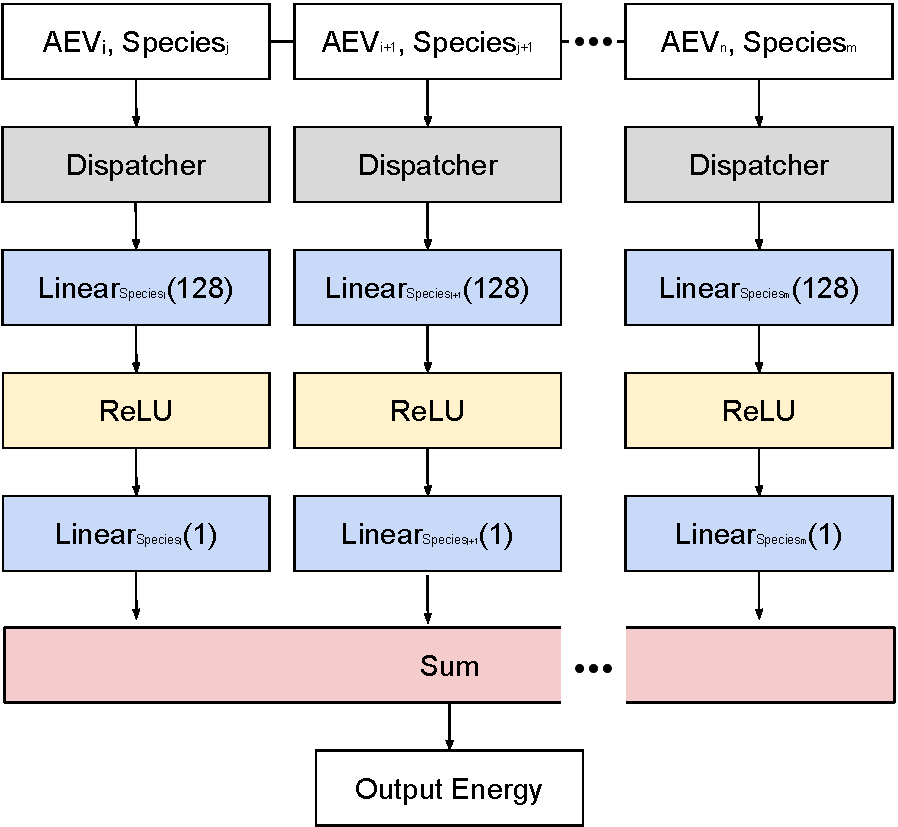
\includegraphics[width=\columnwidth]{figures/bioe142-fig1.pdf}
    \caption{\textbf{Final Model Architecture.} Input atomic structures are transformed into an unordered collection of AEVs and species Labels based on each individual atom in an input molecule. Each input is then "dispatched" based on the Species label to its corresponding feedforward network (one for each species) and an activated scalar value. The values are then summed together to get the final total energy of the molecule. Note that in this diagram, the Linear Layers are indexed by the identity of the species they model, and the AEVs are indexed by the atom they represent.}
    \label{fig:architecture}
\end{figure}

% \newpage

\begin{figure*}[t]
  \centering
  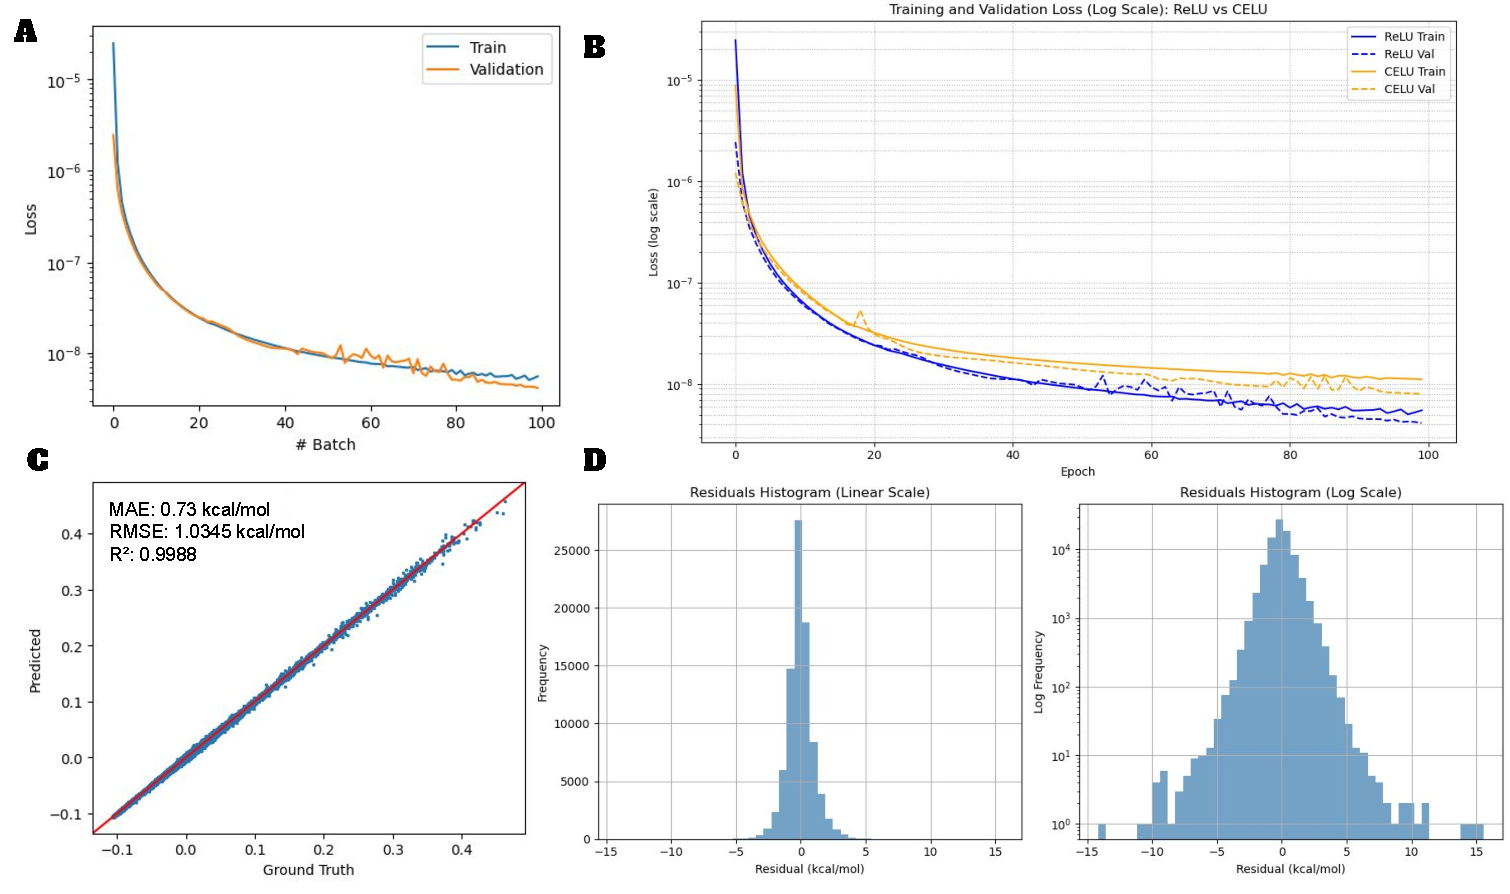
\includegraphics[width=\textwidth]{figures/bioe142-fig2.pdf}
  \caption{\textbf{Training and evaluation results. A.} Training and validation loss curves for the best model during training. The y-axis shows the logged Mean Squared Error (MSE) in hartrees. \textbf{B.} The training and validation loss curves for the best model, and another version that replaced the ReLU activation (blue) with a CeLU activation (yellow). \textbf{C.} A scatterplot of the predicted vs true energies for the unseen test set for the best model, showing a strong linear correlation between the two values and the MAE, RMSE, and $R^2$ values. \textbf{D.} Histograms of the distribution of the residuals for the test set in normal and log scale. The distribution is approximately parametric and centered around 0, suggesting minimal bias.}
  \label{fig:results}
\end{figure*}

My model of the small molecule ANI potential demonstrated excellent performance on the small organic molecule dataset, as evidenced by the comprehensive evaluation metrics presented in Figure 2. Both training and validation loss curves exhibit smooth and consistent convergence throughout the 100 epochs of training. The loss, measured as Mean Squared Error (MSE) on a logarithmic scale, decreased rapidly in the initial epochs and continued to improve gradually. The close alignment between training and validation curves indicates that the model was not overfitting - and in fact likely could have been even more improved with further training on the same dataset due to the final validation loss actually being lower than the training loss. In the source code through 3-fold cross validation I also show that this is likely not an artifact of a lucky split or initialization as similar results were obtained when cross-validating on most folds.

The model achieved remarkable accuracy in predicting molecular energies on the test set, with a Mean Absolute Error (MAE) of 0.73 kcal/mol and a Root Mean Square Error (RMSE) of 1.0345 kcal/mol (Figure 2C). The scatter plot also illustrates very strong linear correlation between predicted and ground truth energies for the unseen test dataset, with an $R^2$ value of 0.9988. This high value also confirms model's excellent predictive capability across the entire energy range of the test molecules. The points align closely with the ideal diagonal line, indicating minimal systematic bias in the predictions. The residual histograms (Figure 2D) provide further insight into the model's error characteristics. The left histogram displays the distribution of residuals on a linear scale, showing a narrow, symmetric distribution centered around zero. This symmetry is particularly important as it indicates the absence of systematic bias in the model's predictions. The majority of prediction errors fall within ±1 kcal/mol, reinforcing the model's chemical accuracy. The right histogram presents the same residual distribution on a logarithmic scale, allowing for better visualization of the tails. This representation reveals that even the largest errors remain within reasonable bounds, with very few outliers. The log-scale histogram confirms that the error distribution is approximately normal, with a slight leptokurtic tendency. These values are well within the chemical accuracy threshold commonly defined as 1 kcal/mol for energy predictions, \cite{bogojeski2020quantum} demonstrating the model's high precision for practical applications in computational chemistry.

\subsection{Practical differences in model fitness based on ReLU vs CeLU activation functions}
Contrary to theoretical expectations, replacing the ReLU activation function with CELU did not improve model performance (Figure 2B). Despite CELU's smoother gradient properties and its potential advantages for gradient flow during backpropagation, the model with ReLU activation (blue curves) consistently outperformed the CELU variant (yellow curves) on both training and validation sets. This result suggests that for this particular application and architecture, the simplicity and computational efficiency of ReLU provided superior performance and that the non-differentiability at zero in ReLU did not appear to hinder gradient-based optimization for this specific task.

\section{Discussion}

\subsection{Position relative to current approaches}

Machine-learning potentials can be roughly divided into descriptor-based models such as ANI that encode symmetry by construction, and message-passing or equivariant graph networks like SchNet \cite{schutt2018schnet} that learn representations end-to-end. Descriptor-based models require less data and train quickly, yet they truncate physics to the descriptor's cutoff; graph networks capture longer-range interactions but are heavier and sometimes harder to train stably on modest hardware. The results indicate that, for compact organic molecules where electronic effects are largely local, a lightweight descriptor plus a shallow network can still meet chemical-accuracy standards—an encouraging sign for resource-constrained applications such as high-throughput ligand scoring or rapid conformer ranking. In fact, the model's performance suggests it can be made even more compact for the current dataset.

\subsection{Limitations}

\paragraph{Label imbalance not addressed.} The GDB-based subset is skewed toward low-energy conformers and certain functional groups; no re-weighting or focal losses were applied.

\paragraph{Near-leakage risk.} Molecules with almost identical chemical structures but slightly different conformers or substituents might land in both train and test sets, exaggerating generalization. A scaffold or energy-stratified split would give a stricter assessment.

\paragraph{Architecture search was minimal.} Multi-head attention, deeper residual stacks, and smoother activations (GELU, CELU) were tested but not tuned exhaustively; hyper-parameter tools (Optuna, Ray Tune) could uncover better settings.

\paragraph{No variations on species-specific networks.} The identical feedforward network for each atom type was a simplification. Work from Stevenson et al. \cite{stevenson2019schr} suggests that different atom types can benefit from different architectures, especially in the context of larger systems. The current model's architecture was designed to be simple and efficient, but it may not fully capture the complexity of interactions between different atom types. Also from a information compression perspective, it is reasonable to assume that different atom types may have different levels of information content, and therefore, some can use less parameters than others to achieve similar performance.

\subsection{Future work}

Addressing the imbalance and leakage issues should be the first priority—e.g.\ clustered cross-validation by Bemis-Murcko scaffolds or conformer families.
Next, incorporating forces into the loss (as done in ANI-1ccX) would enable geometry optimization and molecular-dynamics use. Hybrid approaches that keep the fast AEV descriptor for near-field interactions but append a learned long-range correction, or that swap the feed-forward core for an equivariant message-passing block, could extend accuracy to larger, more polar systems without sacrificing speed.

\section{Code Availability}

All code, data, and pytorch models used in this project are publicly available on GitHub under the MIT license at \url{https://github.com/Qile0317/bioe142-final-project}.

\printbibliography[heading=bibnumbered]

\end{document}
